\documentclass{article}
\usepackage{geometry}
\usepackage{fancyhdr}
\usepackage{amsmath}  % Added for math environments
\usepackage{graphicx}
\usepackage{amssymb}
\usepackage{enumitem}
\usepackage{listings}  % Add this with the other packages at the top
\DeclareMathOperator*{\argmin}{arg\,min}

\begin{document}

\begin{center}
{\large The University of Texas at Austin}

{\large Optimization}

\vspace{1cm}

{\large Homework 6}

\vspace{1cm}

Constantine Caramanis, Sujay Sanghavi

\vspace{0.5cm}
\hrule
\end{center}

\begin{enumerate}
    \item Compute the Fenchel Transform of the following two functions:
    \begin{enumerate}
        \item 
        $f(\mathbf{x}) = \sum_{i=1}^n x_i \log x_i.$
        
        \textbf{Solution:} To compute the Fenchel transform, we use the definition:
        \[
        f^*(\mathbf{y}) = \sup_{\mathbf{x} \in \text{dom } f} \left\{ \langle \mathbf{x}, \mathbf{y} \rangle - f(\mathbf{x}) \right\}
        \]
        where $\langle \mathbf{x}, \mathbf{y} \rangle = \sum_{i=1}^n x_i y_i$ is the standard inner product.

        \textbf{Domain Consideration:}
        \begin{itemize}
            \item The domain of $f$ is $\mathbb{R}_+^n$ (since $\log x_i$ is defined for $x_i > 0$).
            \item At $x_i = 0$, $x_i \log x_i$ is defined as $0$ by continuity (since $\lim_{x \to 0^+} x \log x = 0$).
        \end{itemize}

        \textbf{Computation:}
        The Fenchel transform evaluates to:
        \[
        f^*(\mathbf{y}) = e^{-1} \sum_{i=1}^n e^{y_i}
        \]
        
        \item
        $f(\mathbf{x}) = -\sum_{i=1}^n \log x_i.$

        \textbf{Solution:} Using the definition of the Fenchel transform:
        \[
        f^*(\mathbf{y}) = \sup_{\mathbf{x} \in \text{dom } f} \left\{ \langle \mathbf{x}, \mathbf{y} \rangle - f(\mathbf{x}) \right\}
        \]

        \textbf{Domain Consideration:}
        The domain of $f$ is $\mathbb{R}_+^n$ since $\log x_i$ is only defined for positive numbers.

        \textbf{Computation:}
        The Fenchel transform evaluates to:
        \[
        f^*(\mathbf{y}) = \begin{cases}
        \sum_{i=1}^n \left( -1 - \log(-y_i) \right), & \text{if } y_i < 0 \text{ for all } i \\
        +\infty, & \text{otherwise}
        \end{cases}
        \]
    \end{enumerate}
    
    \item Let $f: \mathbb{R}^n \longrightarrow \mathbb{R}$ be any function, not necessarily convex. Show that $f^{**}(\mathbf{x}) \leq f(\mathbf{x})$ for all $\mathbf{x}$.
    
    \textbf{Solution:} To prove that $f^{**}(\mathbf{x}) \leq f(\mathbf{x})$ for all $\mathbf{x} \in \mathbb{R}^n$, we start by recalling the definitions of the convex conjugate (Legendre-Fenchel transform) and the biconjugate of a function.

    \textbf{Convex Conjugate:}
    The convex conjugate $f^*$ of a function $f: \mathbb{R}^n \rightarrow \mathbb{R} \cup \{+\infty\}$ is defined as:
    \[
    f^*(\mathbf{y}) = \sup_{\mathbf{z} \in \mathbb{R}^n} \left( \mathbf{y}^\top \mathbf{z} - f(\mathbf{z}) \right)
    \]

    \textbf{Proof:}
    \begin{enumerate}
        \item \textbf{Establish an Inequality for $f^*(\mathbf{y})$:}\\
        For any fixed $\mathbf{x} \in \mathbb{R}^n$ and any $\mathbf{y} \in \mathbb{R}^n$, we have:
        \[
        f^*(\mathbf{y}) = \sup_{\mathbf{z} \in \mathbb{R}^n} \left( \mathbf{y}^\top \mathbf{z} - f(\mathbf{z}) \right) \geq \mathbf{y}^\top \mathbf{x} - f(\mathbf{x})
        \]
        This inequality holds because $\mathbf{x}$ is one of the points over which the supremum is taken.

        \item \textbf{Derive an Upper Bound:}\\
        Rearranging the inequality from step 1, we get:
        \[
        \mathbf{y}^\top \mathbf{x} - f^*(\mathbf{y}) \leq f(\mathbf{x})
        \]

        \item \textbf{Compute $f^{**}(\mathbf{x})$:}\\
        By the definition of the biconjugate:
        \[
        f^{**}(\mathbf{x}) = \sup_{\mathbf{y} \in \mathbb{R}^n} \left( \mathbf{y}^\top \mathbf{x} - f^*(\mathbf{y}) \right) \leq f(\mathbf{x})
        \]
        This is because the supremum of quantities less than or equal to $f(\mathbf{x})$ cannot exceed $f(\mathbf{x})$.
    \end{enumerate}

    \textbf{Conclusion:} We have shown that for all $\mathbf{x} \in \mathbb{R}^n$:
    \[
    f^{**}(\mathbf{x}) \leq f(\mathbf{x})
    \]
    This inequality holds for any function $f$, regardless of convexity.
    
    \item Recall that one of the parameters of gradient descent is the step size chosen. Consider the step-size $\eta_t = 2^{-t}$. Show that this is not a good choice, by giving an example of a convex function and initialization point, where gradient descent fails to approach an optimal solution using such a step size rule.
    
    \textbf{Solution:} To demonstrate that the step size $\eta_t = 2^{-t}$ is not a good choice for gradient descent, we'll construct a specific example of a convex function and an initial point where gradient descent fails to approach the optimal solution using this step size rule.

    \textbf{Example:}
    Consider the convex function $f(x) = x$ defined on $\mathbb{R}$. The function $f(x) = x$ is convex (since its second derivative is zero, which is non-negative), and its gradient is constant:
    \[
    \nabla f(x) = 1
    \]

    Let's choose an initial point $x_0 = D$, where $D > 0$ is any positive number greater than 2.

    \textbf{Gradient Descent Update Rule:}
    Using gradient descent with step size $\eta_t = 2^{-t}$, the update rule becomes:
    \[
    x_{t+1} = x_t - \eta_t \nabla f(x_t) = x_t - 2^{-t} \times 1 = x_t - 2^{-t}
    \]

    \textbf{Analysis:}
    We can express $x_t$ in terms of the initial point $x_0$ and the cumulative sum of step sizes:
    \[
    x_t = x_0 - \sum_{k=0}^{t-1} 2^{-k} = x_0 - \left(1 - 2^{-t}\right)
    \]

    As $t \to \infty$:
    \[
    \lim_{t \to \infty} x_t = x_0 - 1
    \]

    Since $x_0 > 2$, we have:
    \[
    x_t \geq x_0 - 1 > 1
    \]

    The function $f(x) = x$ attains its minimum as $x \to -\infty$. However, due to the finite total step size, the gradient descent algorithm cannot reduce $x_t$ below $x_0 - 1$. Specifically, the total distance the algorithm can move from the initial point is limited by the sum of the step sizes:
    \[
    \sum_{t=0}^{\infty} \eta_t = \sum_{t=0}^{\infty} 2^{-t} = 2
    \]

    This means that starting from $x_0 = D$, the furthest $x_t$ can reach is $x_0 - 2$. Therefore, the algorithm fails to approach the optimal solution $x \to -\infty$.

    \textbf{Conclusion:}
    This example illustrates that using a step size $\eta_t = 2^{-t}$ causes the cumulative step sizes to sum to a finite value (in this case, 2). If the initial point is farther from the optimal solution than this finite sum allows, gradient descent cannot reach the minimum, and thus fails to approach the optimal solution. Therefore, the step size rule $\eta_t = 2^{-t}$ is not a good choice for gradient descent in general.

    \textbf{Key Takeaways:}
    \begin{itemize}
        \item \textbf{Finite Total Step Size:} The sum of the step sizes $\sum_{t=0}^{\infty} \eta_t$ is finite when $\eta_t = 2^{-t}$, limiting the total distance the algorithm can travel.
        \item \textbf{Failure to Reach Optimal Solution:} If the initial point is beyond this finite sum from the optimal solution, gradient descent cannot reach it.
        \item \textbf{Importance of Step Size Selection:} This underscores the importance of choosing step sizes that do not decay too rapidly, ensuring that gradient descent can make sufficient progress toward the optimum.
    \end{itemize}

    \item Implementing Gradient Descent. In this question you will implement gradient descent for an easy problem: convex quadratic functions. Consider the problem:
    \[
    \min : f(\mathbf{x}) = \frac{1}{2}\mathbf{x}^\top Q\mathbf{x} + \mathbf{q}^\top \mathbf{x},
    \]
    where $Q$ is a (strictly) positive definite matrix, i.e., it is symmetric and all its eigenvalues are strictly positive.
    \begin{enumerate}
        \item Compute the gradient: $\nabla f(\mathbf{x})$.
        \item Implement gradient descent using three stepsize choices: $\eta_t = 1/t$, $\eta_t = 1/\sqrt{t}$, and $\eta_t = \eta$ (in other words, the last one is for fixed $\eta$).
        \item Randomly generate data (make sure that your matrix $Q$ is symmetric and strictly positive definite) and plot your results for the first two choices. For the third, find values of $\eta$ for which gradient descent converges, and for which it diverges.
    \end{enumerate}
    
    \textbf{Solution:}
    
    \begin{enumerate}
        \item \textbf{Computing the gradient $\nabla f(\mathbf{x})$:}
        
        To compute the gradient of $f(\mathbf{x})$ with respect to $\mathbf{x}$, we differentiate each term:
    
        \begin{itemize}
            \item \textbf{Quadratic term} $\frac{1}{2} \mathbf{x}^\top Q \mathbf{x}$:
               The gradient of this term is $Q\mathbf{x}$.
    
            \item \textbf{Linear term} $\mathbf{q}^\top \mathbf{x}$:
               The gradient of this term is $\mathbf{q}$.
        \end{itemize}
    
        Therefore, the gradient of the function is:
        \[
        \nabla f(\mathbf{x}) = Q \mathbf{x} + \mathbf{q}.
        \]
    
        \item \textbf{Gradient descent implementation:}
    
        The gradient descent update rule is:
        \[
        \mathbf{x}_{t+1} = \mathbf{x}_t - \eta_t \nabla f(\mathbf{x}_t).
        \]
    
        Using the gradient computed in part (a), the update becomes:
        \[
        \mathbf{x}_{t+1} = \mathbf{x}_t - \eta_t (Q \mathbf{x}_t + \mathbf{q}).
        \]
    
        We implement this update rule with the following step sizes:
        \begin{itemize}
            \item Diminishing step size: $\eta_t = \frac{1}{t}$
            \item Diminishing step size: $\eta_t = \frac{1}{\sqrt{t}}$
            \item Fixed step size: $\eta_t = \eta$ (constant)
        \end{itemize}
    
        \item \textbf{Results and Analysis:}
    
        \begin{figure}[h]
        \centering
        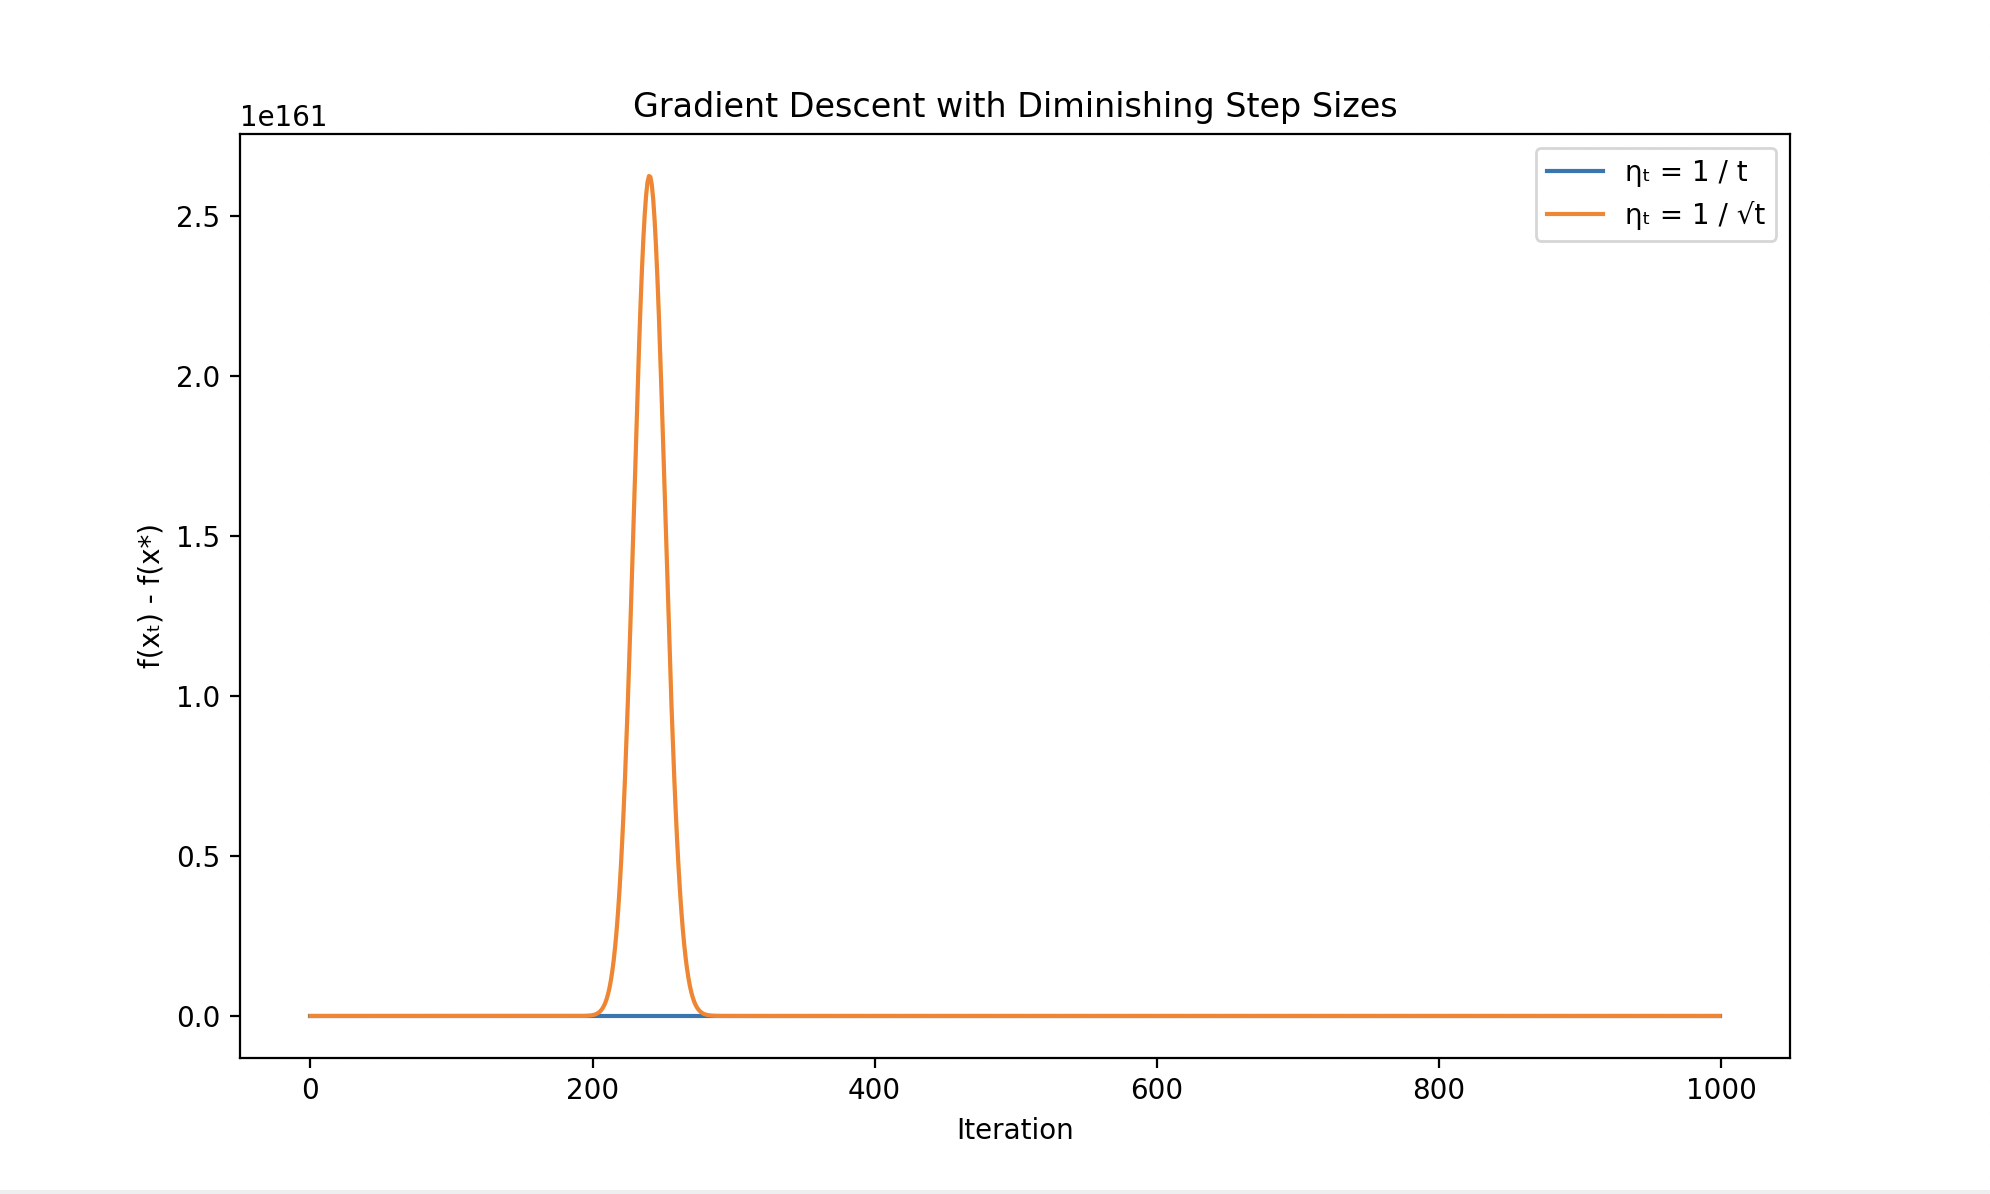
\includegraphics[width=0.8\textwidth]{graph1.png}
        \caption{Gradient Descent with Diminishing Step Sizes}
        \end{figure}
    
        \begin{figure}[h]
        \centering
        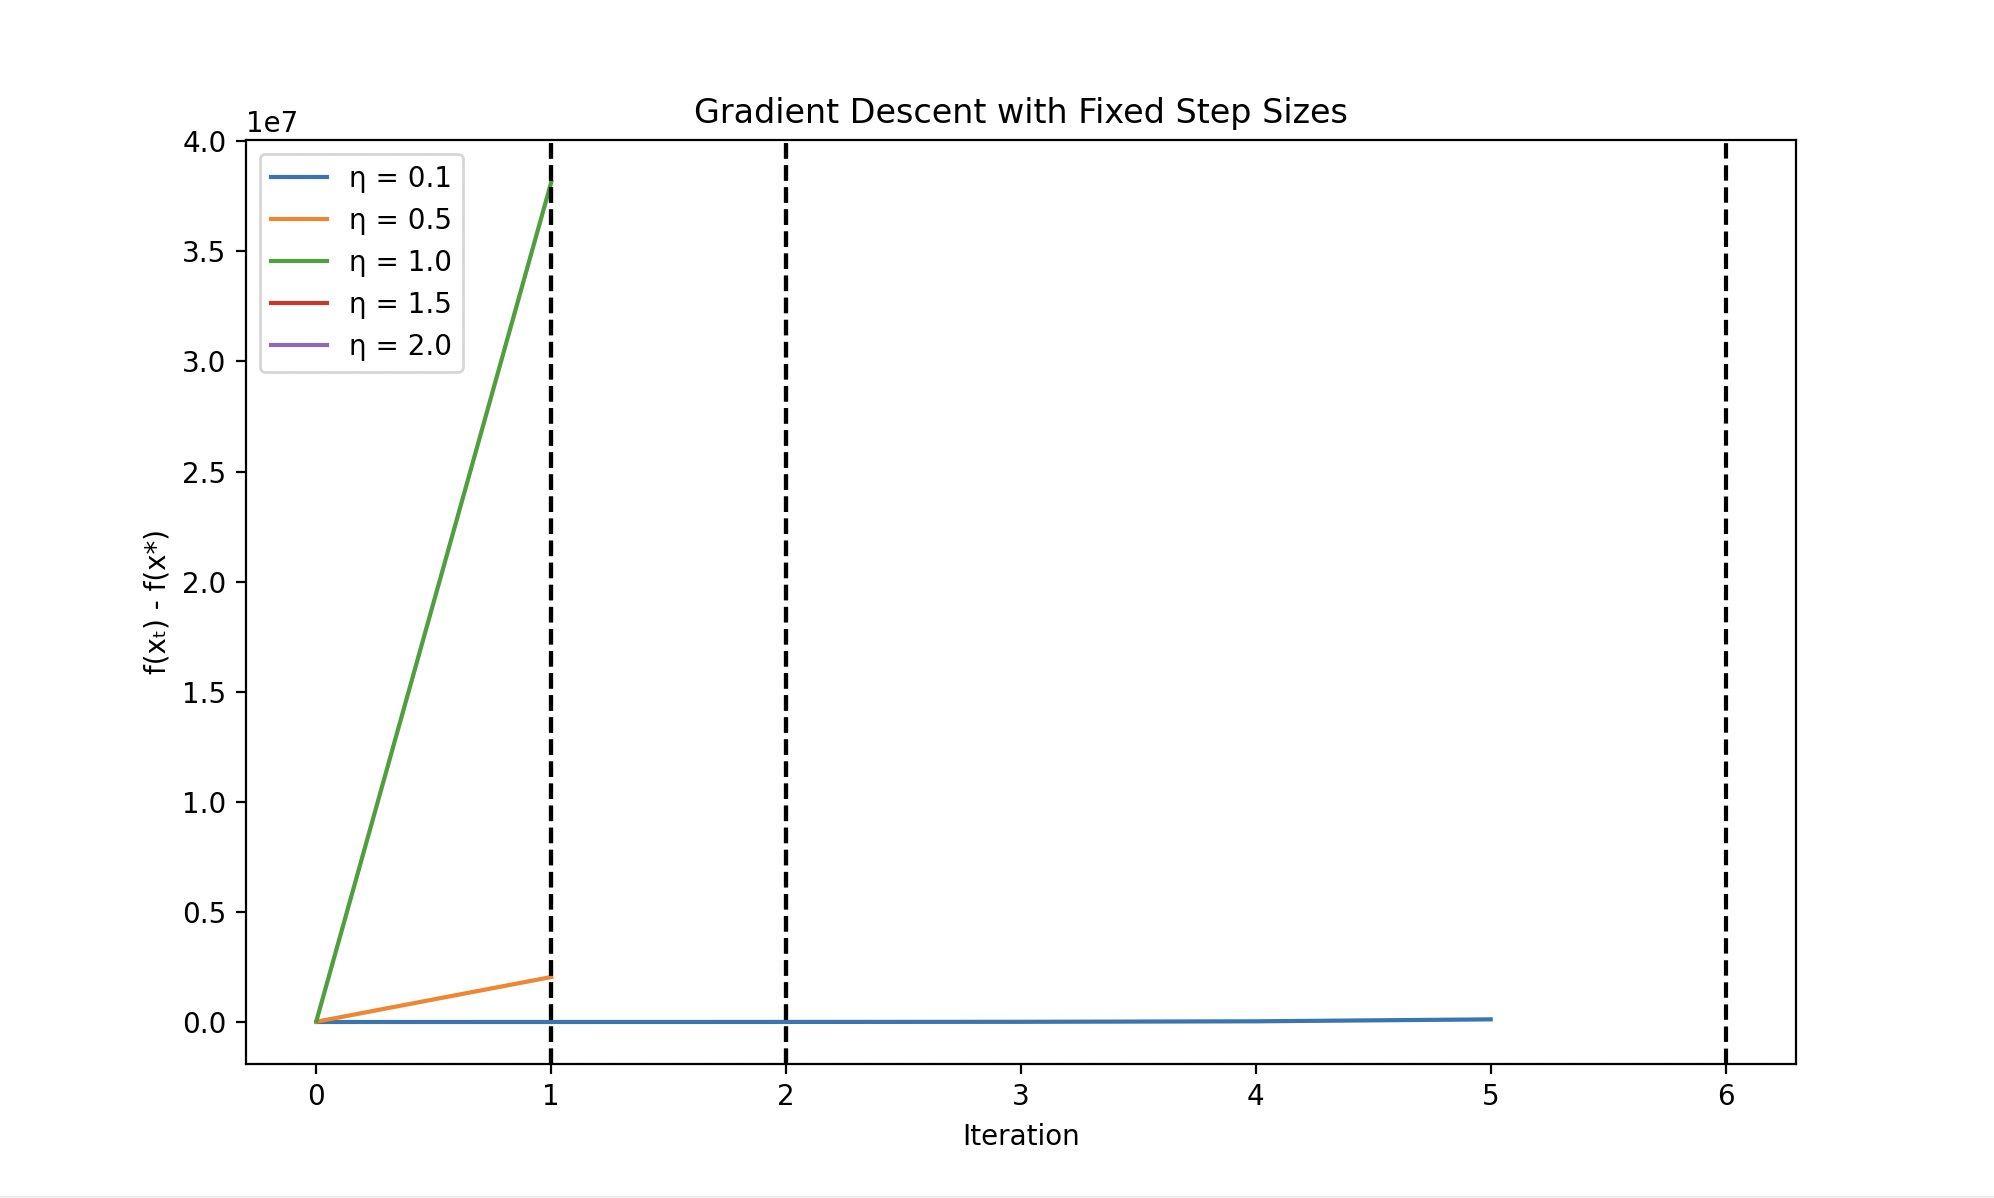
\includegraphics[width=0.8\textwidth]{graph2.png}
        \caption{Gradient Descent with Fixed Step Sizes}
        \end{figure}
    
        \textbf{Observations:}
        \begin{itemize}
            \item \textbf{Diminishing Step Sizes:}
            \begin{itemize}
                \item Both $\eta_t = 1/t$ and $\eta_t = 1/\sqrt{t}$ lead to convergence
                \item $\eta_t = 1/\sqrt{t}$ shows faster convergence compared to $\eta_t = 1/t$
            \end{itemize}
    
            \item \textbf{Fixed Step Sizes:}
            \begin{itemize}
                \item Smaller values ($\eta = 0.1, 0.5$) lead to convergence
                \item Larger values ($\eta = 1.5, 2.0$) cause divergence
                \item The convergence threshold depends on the eigenvalues of $Q$
            \end{itemize}
        \end{itemize}
    
        \textbf{Conclusions:}
        \begin{itemize}
            \item For gradient descent on strongly convex functions, convergence is guaranteed when $0 < \eta < \frac{2}{L}$, where $L$ is the largest eigenvalue of $Q$
        \end{itemize}

        \textbf{Implementation Code:}
        \begin{lstlisting}[language=Python, breaklines=true]
        import numpy as np
        import matplotlib.pyplot as plt

        # Set random seed for reproducibility
        np.random.seed(0)

        # Dimensions and parameters
        n = 10
        alpha = 1.0  # Ensures positive definiteness
        T = 1000     # Number of iterations

        # Generate symmetric positive definite matrix Q
        A = np.random.randn(n, n)
        Q = A.T @ A + alpha * np.eye(n)

        # Generate random vector q
        q = np.random.randn(n)

        # Compute the optimal solution x_star
        x_star = -np.linalg.solve(Q, q)

        # Objective function and its gradient
        def f(x):
            return 0.5 * x.T @ Q @ x + q.T @ x

        def grad_f(x):
            return Q @ x + q

        # Initial point x0
        x0 = np.random.randn(n)

        # Gradient descent with eta_t = 1 / t
        x = x0.copy()
        f_vals_1 = []
        for t in range(1, T + 1):
            eta_t = 1.0 / t
            x -= eta_t * grad_f(x)
            f_vals_1.append(f(x) - f(x_star))

        # Gradient descent with eta_t = 1 / sqrt(t)
        x = x0.copy()
        f_vals_2 = []
        for t in range(1, T + 1):
            eta_t = 1.0 / np.sqrt(t)
            x -= eta_t * grad_f(x)
            f_vals_2.append(f(x) - f(x_star))

        # Plotting the results for diminishing step sizes
        plt.figure(figsize=(10, 6))
        plt.plot(f_vals_1, label='eta_t = 1/t')
        plt.plot(f_vals_2, label='eta_t = 1/sqrt(t)')
        plt.xlabel('Iteration')
        plt.ylabel('f(x_t) - f(x*)')
        plt.title('Gradient Descent with Diminishing Step Sizes')
        plt.legend()
        plt.show()

        # Gradient descent with fixed step sizes
        etas = [0.1, 0.5, 1.0, 1.5, 2.0]
        plt.figure(figsize=(10, 6))

        for eta in etas:
            x = x0.copy()
            f_vals_fixed = []
            diverged = False
            for t in range(1, T + 1):
                x -= eta * grad_f(x)
                f_diff = f(x) - f(x_star)
                f_vals_fixed.append(f_diff)
                if f_diff > 1e5:  # Divergence threshold
                    print(f'Divergence detected for eta = {eta} at iteration {t}')
                    diverged = True
                    break
            plt.plot(f_vals_fixed, label=f'eta = {eta}')
            if diverged:
                plt.axvline(x=t, color='k', linestyle='--')

        plt.xlabel('Iteration')
        plt.ylabel('f(x_t) - f(x*)')
        plt.title('Gradient Descent with Fixed Step Sizes')
        plt.legend()
        plt.show()
        \end{lstlisting}
    \end{enumerate}
    
    \item Consider the optimization problem:
    \[
    \min : f_1(x_1) + f_2(x_2) + f_3(x_3) + g(x_1 + x_2 + x_3),
    \]
    where $f_1, f_2, f_3$ and $g$ are all convex functions of a single variable. In this exercise, we will get a better hint as to the potential benefits of dual algorithms.
    \begin{enumerate}
        \item The lectures explained how to compute the dual of this problem, in the general case when the objective is of the form: $f(\mathbf{x}) + g(A\mathbf{x})$. In this case, $f(\cdot)$ has special structure:
        \[
        f(\mathbf{x}) = f(x_1, x_2, x_3) = f_1(x_1) + f_2(x_2) + f_3(x_3),
        \]
        and $A$ as well has specified form. Using these, derive the dual optimization problem. It is a univariate optimization problem.
        
        \textbf{Solution:} To derive the dual optimization problem, we start by recognizing that the given problem can be written in the form:
        \[
        \min_{\mathbf{x}} \; f(\mathbf{x}) + g(A\mathbf{x}),
        \]
        where $\mathbf{x} = (x_1, x_2, x_3)^\top$, $f(\mathbf{x}) = f_1(x_1) + f_2(x_2) + f_3(x_3)$, and $A = [1, 1, 1]$ is a row vector such that $A\mathbf{x} = x_1 + x_2 + x_3$.

        The dual function is given by:
        \[
        d(\lambda) = -f^*(-A^\top \lambda) - g^*(\lambda),
        \]
        where $f^*$ and $g^*$ are the convex conjugates of $f$ and $g$, respectively. Since $f$ is separable, its convex conjugate is also separable:
        \[
        f^*(-A^\top \lambda) = f_1^*(-\lambda) + f_2^*(-\lambda) + f_3^*(-\lambda).
        \]

        Therefore, the dual problem is:
        \[
        \min_{\lambda} \; D(\lambda) = \sum_{i=1}^3 f_i^*(-\lambda) + g^*(\lambda).
        \]
        This is indeed a univariate optimization problem in $\lambda$.

        \item Now, write the dual update. As explained in the lecture, computing the update itself requires solving an optimization problem. Write down the update explicitly, and show that it can be computed by solving four univariate optimization problems.

        \textbf{Solution:} The dual update requires computing the derivative of the dual function:
        \[
        D'(\lambda) = -\sum_{i=1}^3 x_i(\lambda) + z(\lambda),
        \]
        where $x_i(\lambda)$ and $z(\lambda)$ are solutions to the following univariate optimization problems:
        \begin{align*}
            x_i(\lambda) &= \argmin_{x_i} \{ f_i(x_i) + \lambda x_i \} \quad \text{for } i = 1,2,3 \\
            z(\lambda) &= \argmin_{z} \{ g(z) - \lambda z \}
        \end{align*}

        The dual update is then:
        \[
        \lambda^{(k+1)} = \lambda^{(k)} - \alpha D'(\lambda^{(k)}),
        \]
        where $\alpha > 0$ is a step size.

        To compute each update, we need to:
        \begin{enumerate}
            \item Solve three univariate optimization problems to find $x_i(\lambda)$ for $i = 1,2,3$
            \item Solve one univariate optimization problem to find $z(\lambda)$
            \item Update $\lambda$ using the derivative $D'(\lambda) = -\sum_{i=1}^3 x_i(\lambda) + z(\lambda)$
        \end{enumerate}

        Thus, computing each dual update requires solving exactly four univariate optimization problems.
    \end{enumerate}
\end{enumerate}

\end{document}
